\chapter{Methodology}

This study employs a quantitative approach to analyze labor force participation rates across all 50 U.S. states from 1976 to 2020. Data on labor force participation rates were sourced from The Federal Reserve Bank of St. Louis Fed\footnote{Federal Reserve Bank of St. Louis. (n.d.). Civilian labor force participation rate [CIVPART]. Federal Reserve Bank of St. Louis. Retrieved November 11, 2024, from \href{https://fred.stlouisfed.org/series/CIVPART}{https://fred.stlouisfed.org/series/CIVPART}}, while information regarding the political affiliation of each state's governor during this period was compiled into a binary variable, where 1 indicates a Democratic governor and 0 indicates a Republican governor, with the data obtained from Open ICPSR. Additionally, population figures for each state, essential for calculating weighted participation rates, were retrieved from The United States Census Bureau. To compute the weighted labor force participation rates, the study utilized the formula:

\begin{equation}
\text{Weighted Mean} = \frac{\sum (\text{Participation Rate} \times \text{Population})}{\sum \text{Population}}
\end{equation}

As well as a model of the regression analysis:
\begin{equation}

\text{Labor Force Participation Rate} = \beta_0 + \beta_1 \times \text{Democratic Governor} + \epsilon
\end{equation}

To conduct the regression analysis, Python was employed, utilizing libraries such as \texttt{pandas} and \texttt{statsmodels}. The weighted least squares (WLS) method was applied to account for population size, with rigorous checks for linearity, independence, homoscedasticity, and normality of residuals. This methodology provides a comprehensive framework to assess the impact of political governance on labor force participation across the states, facilitating a nuanced understanding of the relationship between governance and workforce engagement.

\textbf{Labor Force Participation Rate (national) Data -- from FRED}

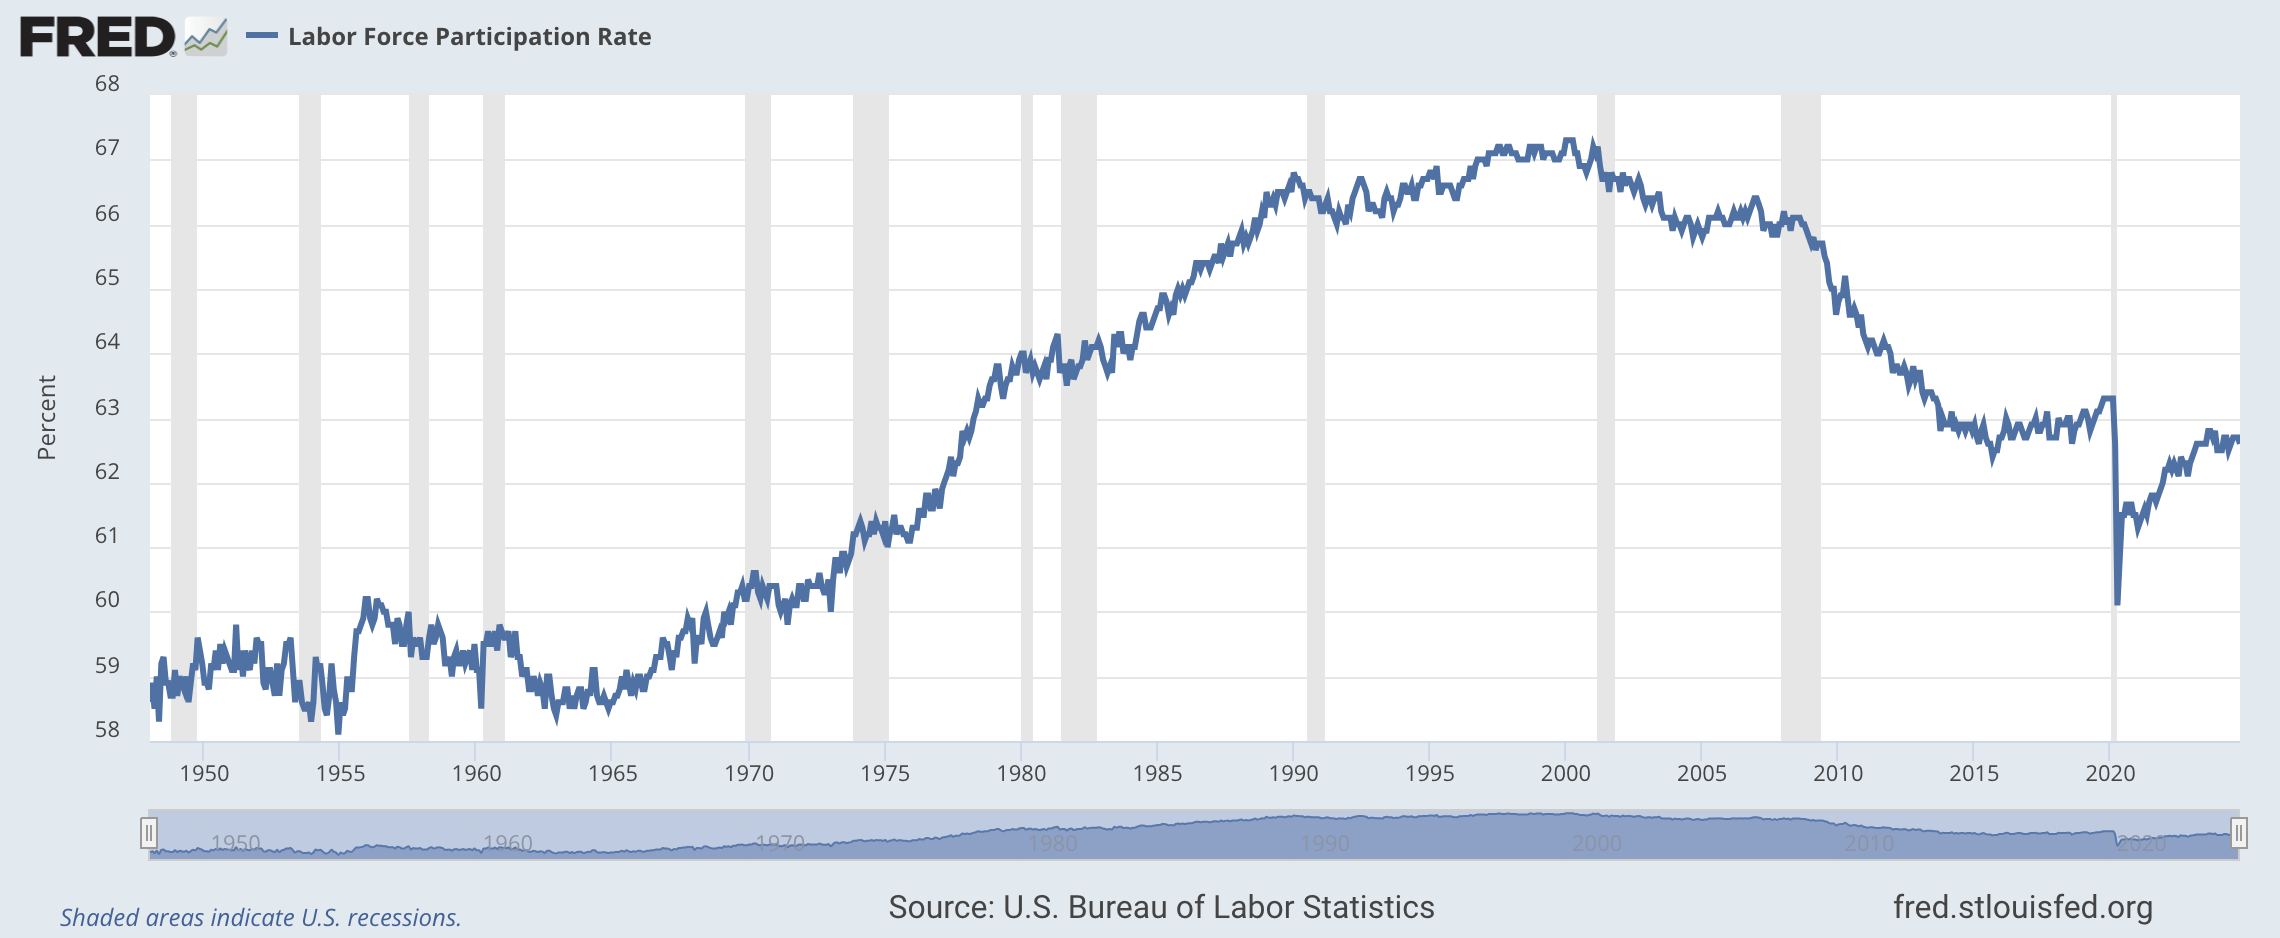
\includegraphics[width=0.7\linewidth]{files/FRED-b4c4bb880b38d58a7677f8cacc531c46.png}

\textbf{Weighted Mean Calculations}

\begin{verbatim}
import pandas as pd

# Load data from a CSV file
df = pd.read_csv('/home/idies/workspace/Temporary/ymettawa/scratch/as.180.369/contrib/yazzymettawa/Paper_Final/Data/stateLFPR.csv')  # Replace 'data.csv' with your actual file path

# Calculate weighted mean for each party
weighted_means = (
    df.assign(Weighted_Participation=df['number'] * df['population'])
    .groupby('party')
    .agg(Weighted_Mean=('Weighted_Participation', 'sum'),
         Total_Population=('population', 'sum'))
    .reset_index()
)

# Calculate final weighted mean
weighted_means['Weighted_Mean'] = weighted_means['Weighted_Mean'] / weighted_means['Total_Population']

# Map party numbers to names
weighted_means['party'] = weighted_means['party'].map({0: 'Republican', 1: 'Democratic'})
# Drop unnecessary columns
weighted_means = weighted_means[['party', 'Weighted_Mean']]

# Print the results
print(weighted_means)
\end{verbatim}

\begin{verbatim}
party  Weighted_Mean
0  Republican      65.486649
1  Democratic      65.188772
\end{verbatim}

\textbf{State Level WLS Regression}

\begin{verbatim}
import pandas as pd
import statsmodels.api as sm
import warnings

# Load data from a CSV file
df = pd.read_csv('/home/idies/workspace/Temporary/ymettawa/scratch/as.180.369/contrib/yazzymettawa/Paper_Final/Data/stateLFPR.csv')  # Replace 'data.csv' with your actual file path

# Define the dependent variable (Y) and independent variable (X)
Y = df['number']
X = df['party']  # Use the Party as a binary variable for regression

# Add a constant to the model
X = sm.add_constant(X)

# Fit the weighted regression model
weights = df['population']  # Use population as weights

# Check for the number of observations
if len(df) >= 8:
    model = sm.WLS(Y, X, weights=weights).fit()
    print(model.summary())
else:
    with warnings.catch_warnings():
        warnings.simplefilter("ignore")
        model = sm.WLS(Y, X, weights=weights).fit()
        print(model.summary())
\end{verbatim}

\begin{verbatim}
WLS Regression Results                            
==============================================================================
Dep. Variable:                 number   R -squared:                       0.002
Model:                            WLS   Adj. R -squared:                  0.001
Method:                 Least Squares   F -statistic:                     3.544
Date:                Fri, 06 Dec 2024   Prob (F -statistic):             0.0599
Time:                        13:39:01   Log -Likelihood:                -5336.4
No. Observations:                1839   AIC:                         1.068e+04
Df Residuals:                    1837   BIC:                         1.069e+04
Df Model:                           1                                         
Covariance Type:            nonrobust                                         
==============================================================================
                 coef    std err          t      P>|t|      [0.025      0.975]
 - - - - - - - - - - - - - - - - - - - - - - - - - - - - - - - - - - - - - - - - - - - - - - - - - - - - - - - - - - - - - - - - - - - - - - - - - - - - - -
const         65.4866      0.109    602.302      0.000      65.273      65.700
party         -0.2979      0.158     -1.882      0.060      -0.608       0.012
==============================================================================
Omnibus:                      231.480   Durbin -Watson:                   1.596
Prob(Omnibus):                  0.000   Jarque -Bera (JB):              370.087
Skew:                          -0.865   Prob(JB):                     4.33e -81
Kurtosis:                       4.356   Cond. No.                         2.56
==============================================================================

Notes:
[1] Standard Errors assume that the covariance matrix of the errors is correctly specified.
\end{verbatim}

\textbf{Interpretting the Results}
Examine the coefficents
\begin{equation}

\beta_1 \text{> 0 = states with Democratic governors have higher LFPR}
\end{equation}

\begin{equation}
\beta_1 \text{< 0 = states with Democratic governors have lower LFPR}
\end{equation}

Statistical Significance: Look at the p-values associated with your coefficients to determine if the results are statistically significant (typically, p \textless  0.05).
Model Fit: Check the R-squared value to see how much of the variance in labor force participation is explained by your model.

\textbf{National Level OLS Regression}

\begin{verbatim}
import pandas as pd
import statsmodels.api as sm

def ols_regression(csv_file):
    # Load the CSV file into a DataFrame
    df = pd.read_csv(csv_file)

    # Extract the necessary columns: 'CIVPART' and 'Party'
    X = df.iloc[:, 4]  # Party column (5th column)
    y = df.iloc[:, 1]  # CIVPART column (2nd column)

    # Add a constant to the model for the intercept term
    X = sm.add_constant(X)

    # Fit the OLS regression model
    model = sm.OLS(y, X).fit()

    # Print the summary of the regression results
    print(model.summary())

# Example usage:
ols_regression('/home/idies/workspace/Temporary/ymettawa/scratch/as.180.369/contrib/yazzymettawa/Paper_Final/Data/nationalLFPR.csv')
\end{verbatim}

\begin{verbatim}
OLS Regression Results                            
==============================================================================
Dep. Variable:                CIVPART   R -squared:                       0.000
Model:                            OLS   Adj. R -squared:                 -0.001
Method:                 Least Squares   F -statistic:                    0.1830
Date:                Fri, 06 Dec 2024   Prob (F -statistic):              0.669
Time:                        13:39:04   Log -Likelihood:                -2023.5
No. Observations:                 816   AIC:                             4051.
Df Residuals:                     814   BIC:                             4060.
Df Model:                           1                                         
Covariance Type:            nonrobust                                         
==============================================================================
                 coef    std err          t      P>|t|      [0.025      0.975]
 - - - - - - - - - - - - - - - - - - - - - - - - - - - - - - - - - - - - - - - - - - - - - - - - - - - - - - - - - - - - - - - - - - - - - - - - - - - - - -
const         63.1123      0.132    478.078      0.000      62.853      63.371
Party          0.0880      0.206      0.428      0.669      -0.316       0.492
==============================================================================
Omnibus:                    10216.381   Durbin -Watson:                   0.005
Prob(Omnibus):                  0.000   Jarque -Bera (JB):               72.909
Skew:                          -0.184   Prob(JB):                     1.47e -16
Kurtosis:                       1.583   Cond. No.                         2.46
==============================================================================

Notes:
[1] Standard Errors assume that the covariance matrix of the errors is correctly specified.
\end{verbatim}

\section{Results}

Returning to the research question: ``How does the labor force participation rate from the 1953 until 2020 in the United States vary with political party governance" the results suggest that there is little evidence to support a strong or reliable relationship between political party governance and labor force participation rates. This was found to be the case when observing both national political party governance (through the president's party affiliation and state labor force participation rates) as well on the state level (through the governor's party affiliation and state labor force participation rates). However, on the state level the tendency was for participation rates to be higher during Democrat governorships, while on the national level the tendency was for participation rates to be higher during Republican presidencies further undermining any relationship.

\textbf{State Level}

The WLS regression results indicate a  weak relationship between the independent variable (party) and the dependent variable (labor force participation rate). The effect of ``party'' is marginally statistically significant (p $\approx$ 0.06), but the overall model fit is very poor (R\textsuperscript{2} $\approx$ 0.002). The low R-squared value indicates that the predictor ``party'' explains almost none of the variance in ``number.''

\begin{equation}
\text{STATE CIVPART} = 65.4866 + -0.2979 \times \text{Party}
\end{equation}

\textbf{National Level}

The OLS regression results indicate a  weak relationship between the independent variable (party) and the dependent variable (labor force participation rate). The effect of ``party'' is marginally statistically significant (p $\approx$ 0.669), but the overall model fit is very poor (with an adjusted R\textsuperscript{2} $\approx$ -0.001). The low R-squared value indicates that the predictor ``party'' explains almost none of the variance in ``number.''

\begin{equation}
\text{NATIONAL CIVPART} = 63.1123 + 0.0880 \times \text{Party}
\end{equation}

\section{Discussion}

\textbf{Limitations and Next Steps}

Some limitations of the analysis include the simplicity of the econometric approach, which may not fully capture the complexity of political dynamics. Additionally, the political party in power does not necessarily indicate the effect of a policy, as the impact of a policy may only become evident once a different party assumes control. The analysis also excluded third parties for the sake of simplicity, focusing only on the governor and president as key political offices, while not considering the roles of the Senate and House of Representatives. A more meaningful approach might involve analyzing specific policies to assess their impact on participation rates, and then examining which parties supported or opposed those policies to better understand their effects.